\documentclass[logo,reportComp]{thesis}
\usepackage[cpp,pseudo]{mypackage}

\title{分布式系统作业三}
\subtitle{远程过程调用}
\school{数据科学与计算机学院}
\author{陈鸿峥}
\classname{17大数据与人工智能}
\stunum{17341015}
\headercontext{分布式系统作业}

\begin{document}

\maketitle

\begin{question}
远程过程调用(RPC)用将网络编程变得非常简单。
根据所学的RPC相关原理,实现客户端-服务器通信,并进行简单的计算如数据库查询、算术计算、数据挖掘、深度学习推导等。
\begin{figure}[H]
\centering
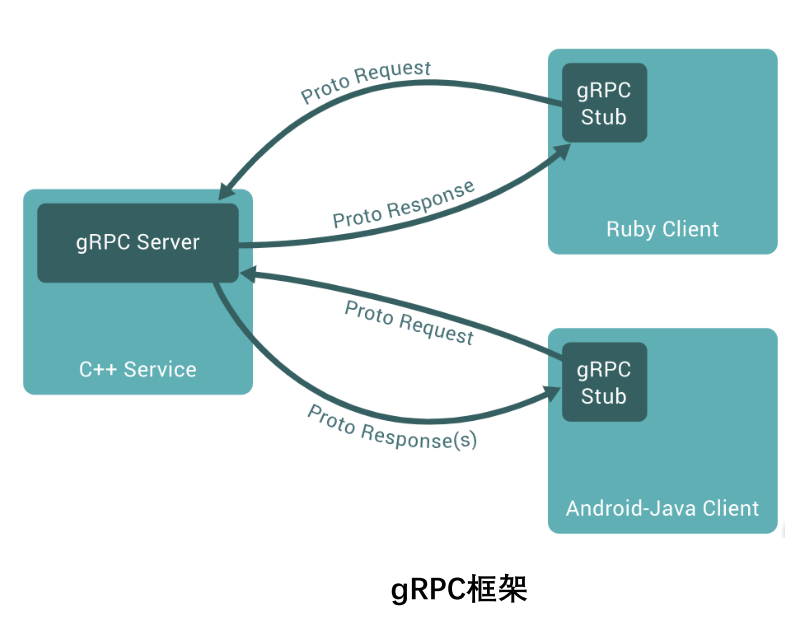
\includegraphics[width=0.6\linewidth]{fig/gRPC-framework.png}
\end{figure}
\begin{itemize}
\item 要求:
\begin{enumerate}
\item 采用gRPC
\item 采用Protobuf作为C-S数据传输格式
\item 服务器端采用线程池,支持并发
\item 支持至少两种的计算服务如简单的算术运算+数据挖掘算法(K-means、KNN等)
\item 编程语言不做要求
\end{enumerate}
\item 建议:gRPC和Protobuf在配置环境时可能有些复杂,对于有些编程语言如C++、Go等会有一些挑战,Python问题会少一些。
\item 关于gRPC的相关例子:\url{https://github.com/grpc/grpc/tree/master/examples}
\end{itemize}
\end{question}

\section{解决方案}

\section{实验结果}

\section{遇到的问题及解决方法}

% \begin{thebibliography}{99}
% \end{thebibliography}

\end{document}